\cleardoublepage
\chapter{外文翻译}
\section*{摘要}
\par 短时降水预测的目的是在较短的时间内预测局部地区未来的降雨强度。过去少有研究从机器学习的角度来研究这个至关重要且具有挑战性的天气预报问题。本文将短时降水预测问题表述为输入和预测目标均为时空序列的时空序列预测问题。通过扩展全连接长短期记忆网络(FC-LSTM),使其在输入到状态和状态到状态的转换中都具有卷积结构,我们提出了卷积长短期记忆网络(ConvLSTM),并将其用于构建短时降水预测问题的端到端可训练模型。实验表明,我们的卷积长短期记忆网络能够更好地捕捉时空相关性,并始终优于全连接长短期记忆网络和最先进的操作ROVER算法。

\section{引言}
\par 长期以来,对短时对流降水的预报一直是天气预报领域的一个重要问题。这项任务的目标是在相对较短的时间内(如0至6小时)对局部地区的降雨强度给予精确和及时的预测。这对于采取及时措施如生成社会层面的紧急降雨警报、为机场制作天气指导以及与较长期的数值天气预报(NWP)模型无缝连接等方面至关重要。由于所需的预报分辨率和时间精度远远高于诸如周平均气温预报的其它传统预报任务,因此短时降水预测问题具有相当大的挑战性,已成为气象学界的一个热门研究课题[22]。

\par 现有的短时降水预测方法大致可以分为两类[22],即基于NWP的方法和基于雷达回波外推的方法。对于NWP方法,其在现在的预报时间尺度上进行预测需要对大气模型中的物理方程进行复杂而细致的模拟。因此,目前最先进的运行中的降水预报系统[19, 6]经常采用更快、更准确的基于雷达回波外推的方法。具体来说,一些计算机视觉技术,特别是基于光流的方法,已经被证明有助于对雷达图进行精确的外推[10, 6, 20]。沿着这条道路,一个最新进展是香港天文台(HKO)为其短程密集暴雨预警系统(SWIRLS)[15]提出的雷达回波实时光流变异方法(ROVER)算法[25]。ROVER使用[5]中的算法计算连续雷达图的光流,并对假设为静止的流场进行半拉格朗日平流[4]以完成预测。然而,这些基于光流的方法的成功是有限的,因为流量估计步骤和雷达回波推断步骤是分开的,确定模型参数以获得良好的预测性能是很有挑战性的。

\par 这些技术问题可以从机器学习的角度来解决。从本质上讲,短时降水预测是一个时空序列预测问题,以过去的雷达图序列为输入,以固定数量(通常大于1)的未来雷达图序列为输出。然而,无论其具体应用如何,这种学习存在着以下问题。首先,由于时空序列的高维度,特别是当必须进行多步骤预测时,除非预测模型能很好地捕捉数据的时空结构,否则是极为困难的。此外,由于大气层的混乱性,为雷达回波数据建立一个有效的预测模型具有更高的挑战性。

\par 深度学习的最新进展尤其是循环神经网络(RNN)和长短期记忆(LSTM)模型[12, 11, 7, 8, 23, 13, 18, 21, 26],为如何解决这一问题提供了一些有益的启示。根据深度学习方法的基本理念,如果我们有一个合理的端到端模型和足够的数据来训练它,我们就能接近解决这个问题了。由于很容易连续收集大量的雷达回波数据,短时降水预测问题能够满足数据需求。因此,现在需要的是一个合适的模型来进行端到端的学习。在[23]中提出的开创性的LSTM编码器-解码器框架,通过训练时间上串联的LSTM,一个用于输入序列,另一个用于输出序列,为序列到序列的学习问题提供了一个通用框架。[18]中表明对下一个视频帧的预测和中间帧的插值可以通过在量化图像斑块得到的视觉词上建立一个基于RNN的语言模型来完成。他们提出了一个递归卷积神经网络来建立空间关系模型,但该模型只能预测未来的一帧,而且用于状态到状态转换的卷积核的大小被限制为1。他们的工作后来在[21]中得到了跟进,指出了多步骤预测在学习有用表征中的重要性。他们建立了一个LSTM编码器-解码器-预测器模型,该模型同时重建了输入序列并预测了未来序列。虽然他们的方法也可以用来解决我们的时空序列预测问题,但他们的模型所采用的全连接长短期记忆(FC-LSTM)层并没有考虑到空间相关性。

\par 在本文中,我们提出了一种新型的卷积长短期记忆网络(ConvLSTM)用于短时降水预测。我们将短时降水预测视为一个时空序列预测问题,可以在[23]中提出的一般序列到序列的学习框架下进行解决。为了更好地模拟时空关系,我们将全连接长短期记忆网络的思想扩展到卷积长短期记忆网络,在输入到状态和状态到状态的转换中都有卷积结构。通过堆叠多个卷积长短期记忆层并形成一个编码-预测结构,我们可以为降水预报建立一个端到端的可训练模型。为了进行评估,我们创建了一个新的现实生活中的雷达回波数据集,这可以促进进一步的研究,特别是为该问题设计机器学习算法。当对合成的Moving-MNIST数据集[21]和雷达回波数据集进行评估时,我们的卷积长短期记忆网络模型一直优于全连接长短期记忆网络和最先进的操作ROVER算法。

\section{预备知识}
\subsection{短时降水预测公式}
\par 短时降水预测的目的是利用以前观察到的雷达回波序列来预测当地地区(如香港、纽约或东京)未来固定长度的雷达图。在实际应用中,雷达图通常是每隔6-10分钟从天气雷达中获取,并对随后的1-6小时进行预报,即预测未来的6-60帧。从机器学习的角度来看,这个问题可以被看作是一个时空序列预测问题。

\par 假设我们在一个由M行和N列组成的$M \times N$网格代表的空间区域内观察一个动态系统。在网格的每个单元内,有$P$个随时间变化的测量值。因此,任何时候的观测都可以用张量$X \in R^{P\times M\times N}$表示,其中R表示观测特征的域。如果我们定期记录观察结果,我们将得到一连串的张量$\hat{\chi _1}$, $\hat{\chi _2}$, $\dots$, $\hat{\chi _t}$。时空序列预测问题是在给定包括当前观测值在内的前$J$个观测值的情况下,预测未来最可能的长度-K序列:

\begin{equation}
  \hat{\chi _{t+1}}, \dots, \hat{\chi _{t+K}}= \mathop{argmax}\limits_{\chi _{t+1}, \dots, \chi _{t+K}} \mathop{p}(\chi _{t+1}, \dots, \chi _{t+K}|\hat{\chi _{t-J+1}}, \hat{\chi _{t-J+2}}, \dots, \hat{\chi _{t}})\label{EqT1}  
\end{equation}

\par 对于短时降水预测,每个时间戳的观测均为二维雷达回波图。如果我们将地图划分为不重叠的斑块,并将斑块内的像素视为其测量值(见图$\ref{FigT1}$),那么现在的预测问题就成为了一个时空序列的预测问题。

\par 可以注意到,我们的时空序列预测问题与单步时间序列预测问题不同:我们的预测目标是一个包含空间和时间结构的序列。虽然一个长度为K的序列中自由变量的数量可以达到$O(M^K N^K P^K)$,但在实践中我们可以利用可能的预测空间的结构来降低维度,从而使问题变得可行。

\subsection{用于序列建模的长短期记忆网络}
\par 对于通用的序列建模,长短期记忆网络作为一种特殊的循环神经网络结构,在以前的各种研究中被证明是稳定和强大的长距离依赖建模[12, 11, 17, 23]。LSTM的主要创新点是它的存储单元$c_t$,它本质上是一个状态信息的积累器。该单元被几个自参数化的控制门访问、写入和清除。每次有新的输入,如果输入门被激活,其信息将被累积到单元中。另外,如果遗忘门$f_t$开启,过去的单元状态$c_{t-1}$也会在这个过程中被 "遗忘"。最新的单元输出$c_t$是否会被传播到最终状态$h_t$是由输出门$o_t$进一步控制的。使用存储单元和门来控制信息流的一个好处是,梯度将始终被保持于单元中(也被称为恒定误差传送带[12]),防止了过快消失的情况,这是香草循环神经网络模型的一个关键问题[12, 17, 2] 。全连接长短期记忆网络可以看作是长短期记忆网络的一个多变量版本,其中输入、单元输出和状态都是一维向量。在本文中,我们沿用了[11]中对全连接长短期记忆网络的表述。关键方程见下文($ref{Eq2}$),其中'$/circ$'表示Hadamard积。

\begin{equation}
  \begin{split}
    & i_t=\sigma(W_{xi}x_t+W_{hi}h_{t-1}+W_{ci}\circ c_{t-1}+b_i)\\
    & f_t=\sigma(W_{xf}x_t+W_{hf}h_{t-1}+W_{cf}\circ c_{t-1}+b_f)\\
    & c_t=f_t\circ c_{t-1}+i_t\circ \tanh(W_{xc}x_t+W_{hc}h_{t-1}+b_c)\\
    & o_t=\sigma(W_{xo}x_t+W_{ho}h_{t-1}+W_{co}\circ c_{t-1}+b_o)\\
    & h_t=o_t\circ \tanh(c_t)\label{EqT2}
  \end{split}
\end{equation}

\par 多个长短期记忆网络可以被堆叠并在时间上串联起来,形成更复杂的结构。这种模型已经被应用于解决许多现实生活中的序列建模问题[23, 26]。

\begin{figure}
  \begin{center}
    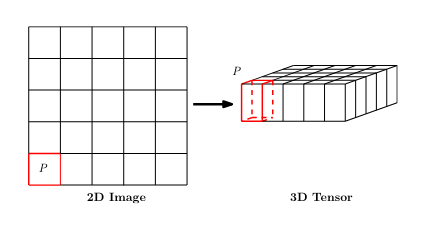
\includegraphics[width=0.8\linewidth]{Figure1.png}
    \caption{二维图像转换至三维张量}
    \label{FigT1}
  \end{center}
\end{figure}